\documentclass[12pt,a4paper]{article}

\usepackage[utf8]{inputenc}
\usepackage[T1]{fontenc}
\usepackage{amsmath,amssymb}
\usepackage{graphicx}
\usepackage{hyperref}
\usepackage{booktabs}
\usepackage[margin=2.5cm]{geometry}
\usepackage{cite}
\usepackage{caption}
\usepackage{subcaption}
\usepackage{float}
\usepackage{xcolor}

\hypersetup{
  colorlinks=true,
  linkcolor=blue,
  citecolor=blue,
  urlcolor=blue
}

\newcommand{\DarkAgents}{DarkAgents}

\title{Minimal Conformal SU(2) Dark Sector and the NANOGrav Signal}

\author{The \DarkAgents{} Collaboration}

\date{June 2026}

\begin{document}

\maketitle

\begin{abstract}
We study the minimal classically scale-invariant SU(2)$_X$ gauge theory with one complex scalar doublet as an explanation of the nanohertz gravitational-wave background reported by NANOGrav. The gauge group is completely broken by the Coleman--Weinberg (CW) mechanism, producing a strongly supercooled first-order phase transition (FOPT). Using the semianalytic pipeline of Ref.~\cite{Pascoli:2026} and the dissipative bulk-flow GW template, we scan the parameter space $g \in [0.1,3.0]$ and $\chi_0 \in [0.1,10000]~\text{GeV}$ and identify 7 benchmark points that achieve 14/14 in-violin bins against the NANOGrav 15-year data. A PTArcade Bayesian campaign yields a maximum a posteriori point at $g = 0.86$, $\chi_0 = 1.12$~GeV, with posterior mean $\langle g \rangle = 0.883 \pm 0.035$ and $\langle \log_{10}(\chi_0/\text{GeV}) \rangle = -0.051 \pm 0.172$. The model is identical to that studied in Ref.~\cite{Borah:2021}, though our analysis uses newer PTA data. The most severe unresolved constraints are $\Delta N_{\text{eff}}$ from the stable dark sector, which contributes up to $\Delta N_{\text{eff}} \sim 0.6$ in the absence of a decay portal, and dark matter overproduction from stable gauge bosons. An audit of 42 assumptions identifies 10 required follow-ups, including dedicated $\Delta N_{\text{eff}}$ and relic abundance calculations. Subject to these caveats, the minimal conformal SU(2) model remains a viable explanation of the PTA signal.
\end{abstract}

\section{Introduction}
\label{sec:intro}

Pulsar timing arrays (PTAs), including NANOGrav~\cite{Agazie:2023}, EPTA, and PPTA, have reported evidence for a stochastic gravitational-wave background (GWB) at nanohertz frequencies. While supermassive black-hole binaries are the canonical source, the spectral index of the signal remains compatible with a broad range of early-universe phenomena, including first-order phase transitions (FOPTs) at the MeV scale.

Classically scale-invariant (conformal) gauge theories provide a compelling, minimal framework for such a FOPT. In these models, the Higgs potential contains no mass term at tree level; the scale of symmetry breaking is generated radiatively via the Coleman--Weinberg (CW) mechanism~\cite{Coleman:1973}. The resulting phase transition is typically strongly supercooled (large latent heat $\alpha$) and slow (moderate $\beta/H$), producing a GW spectrum that can peak in the nanohertz band.

The simplest non-abelian realisation is an SU(2)$_X$ gauge theory with a single complex scalar doublet and no fermions. This model was first studied in the context of NANOGrav by Borah, Dasgupta and Kang~\cite{Borah:2021}. The present work provides an independent analysis using the NANOGrav 15-year data set, the semianalytic pipeline of Ref.~\cite{Pascoli:2026}, and the dissipative bulk-flow (dbf) GW template~\cite{DBFtemplate}. Our companion structurally similar U(1)$'$ study appears in Ref.~\cite{Bringmann:2026}.

The paper is organised as follows. Section~\ref{sec:model} describes the model Lagrangian, particle content, and symmetry-breaking pattern. Section~\ref{sec:fopt} presents the FOPT analysis and scan results. Section~\ref{sec:gw} covers the gravitational-wave spectrum and PTA benchmark comparison. Section~\ref{sec:ptarcade} reports the PTArcade Bayesian analysis. Section~\ref{sec:constraints} summarises constraints. Section~\ref{sec:assumptions} audits the underlying assumptions. We discuss caveats and compare with the literature in Section~\ref{sec:discussion} before concluding in Section~\ref{sec:conclusions}.

\section{The Model}
\label{sec:model}

\subsection{Gauge group and particle content}

The model is a classically scale-invariant SU(2)$_X$ gauge theory containing a complex scalar doublet $\Phi$ and three gauge bosons $W_\mu^a$ ($a=1,2,3$). The field content is summarised in Table~\ref{tab:fields}.

\begin{table}[h]
\centering
\begin{tabular}{lcccc}
\toprule
Field & Type & SU(2)$_X$ rep. & Spin & Real dof \\
\midrule
$\Phi$ & Complex scalar & Fundamental & 0 & 4 \\
$W_\mu^a$ & Gauge boson & Adjoint & 1 & 9 \\
\bottomrule
\end{tabular}
\caption{Particle content of the minimal conformal SU(2)$_X$ model. Four real scalar degrees of freedom from $\Phi$ and three massless gauge bosons ($2\times 3=6$ dof) before SSB; after SSB one radial scalar plus three massive vectors ($3\times3=9$ dof) remain, conserving the total count $4+6=10 = 1+9$.}
\label{tab:fields}
\end{table}

\subsection{Lagrangian}

The tree-level Lagrangian is
\begin{align}
\mathcal{L} &= -\frac14 W_{\mu\nu}^a W^{a,\mu\nu}
+ (D_\mu \Phi)^\dagger (D^\mu \Phi)
- \lambda (\Phi^\dagger \Phi)^2,
\end{align}
where $W_{\mu\nu}^a = \partial_\mu W_\nu^a - \partial_\nu W_\mu^a + g \epsilon^{abc} W_\mu^b W_\nu^c$ and $D_\mu = \partial_\mu + i g W_\mu^a \tau^a$ with $\tau^a = \sigma^a/2$. The potential contains no mass term, reflecting classical scale invariance.

\subsection{Symmetry breaking}

The neutral component of $\Phi$ acquires a vacuum expectation value (VEV) at zero temperature,
\begin{equation}
\langle \Phi \rangle = \frac{1}{\sqrt{2}} \begin{pmatrix} 0 \\ \chi_0 \end{pmatrix},
\end{equation}
which completely breaks SU(2)$_X$ to nothing. Three Goldstone bosons are absorbed as longitudinal modes of the massive gauge bosons, leaving one physical radial scalar $\chi$ (the pseudo-dilaton). The gauge boson mass is
\begin{equation}
m_W = \frac{g\chi_0}{2}.
\end{equation}

\subsection{One-loop effective potential}

At one loop, the CW mechanism generates a non-trivial minimum through gauge-boson loops. The beta-function coefficient for the quartic coupling (in the notation of the backend) is
\begin{equation}
\beta_\lambda = \frac{1}{8\pi^2} \sum_B n_B g_b^4
= \frac{9g^4}{128\pi^2},
\end{equation}
where the sum runs over $9$ real degrees of freedom (three gauge bosons, each with three polarisation states), each with $g_b = g/2$. The radial scalar mass is then
\begin{equation}
m_\chi^2 = \beta_\lambda \,\chi_0^2.
\end{equation}
The zero-temperature vacuum energy difference between the symmetric and broken phases is
\begin{equation}
\Delta V = \frac{\beta_\lambda \,\chi_0^4}{16}.
\end{equation}

\subsection{Free parameters}

The model has two independent parameters:
\begin{itemize}
\item $g \in [0.1, 3.0]$ --- the SU(2)$_X$ gauge coupling,
\item $\chi_0 \in [0.1, 10000]$~GeV --- the scalar VEV at zero temperature.
\end{itemize}

All dimensionful quantities ($m_W$, $m_\chi$, transition temperatures) scale linearly with $\chi_0$. The nHz GW band selects $\chi_0 \sim \mathcal{O}(0.1\text{--}10)$~GeV for perturbative couplings.

\section{First-Order Phase Transition}
\label{sec:fopt}

\subsection{Method}

The finite-temperature effective potential is computed using the high-temperature (small-field) expansion, with the CW zero-temperature potential for the broken-phase minimum. The bounce action $S_3(T)/T$ is obtained via the semianalytic approach of Ref.~\cite{Pascoli:2026}. Percolation is determined using the Gaussian approximation for the false-vacuum fraction, which reduces the percolation temperature to a root-finding problem. The transition strength $\alpha$ (latent heat normalised to radiation energy density) and inverse duration $\beta/H$ are defined in the standard way~\cite{Pascoli:2026}.

\subsection{Scan strategy}

A two-stage scan was performed:
\begin{enumerate}
\item \textbf{Broad grid}: $g \in [0.3, 2.5]$ (12 linear steps), $\chi_0 \in [10^{-4}, 10^{2}]$~GeV (15 log steps) --- 180 points.
\item \textbf{Refined grid}: $g \in [0.7, 2.3]$ (20 linear steps), $\chi_0 \in [3\times10^{-5}, 0.5]$~GeV (25 log steps) --- 500 points.
\end{enumerate}
Total unique points: 680.

\subsection{Results}

Table~\ref{tab:fopt_stats} summarizes the scan outcomes.

\begin{table}[h]
\centering
\begin{tabular}{lrr}
\toprule
Metric & Count & Fraction \\
\midrule
Total points & 680 & 100\% \\
Viable (FOPT occurs) & 482 & 71\% \\
Numerical failures & 174 & 26\% \\
Physical failures & 24 & 3\% \\
In PTA band ($10^{-9}$--$10^{-7}$~Hz) & 187 & 28\% \\
\bottomrule
\end{tabular}
\caption{FOPT scan statistics for the conformal SU(2)$_X$ model.}
\label{tab:fopt_stats}
\end{table}

Viable points span $\alpha \in [0.1, 10^{28}]$, $\beta/H \in [8, 555]$, $T_p \in [10^{-13}, 22]$~GeV, and $T_{\text{reh}} \in [10^{-6}, 23]$~GeV. The PTA-relevant parameter region is $g \in [0.8, 2.3]$, $\chi_0 \in [3\times10^{-5}, 0.5]$~GeV.

\subsection{Comparison with literature}

The benchmark point BP1 of Ref.~\cite{Borah:2021} ($g=1.37$, $\chi_0=0.012$~GeV) was recomputed with our pipeline. Results are compared in Table~\ref{tab:lit_compare}.

\begin{table}[h]
\centering
\begin{tabular}{lccc}
\toprule
Quantity & This work & Borah et al.\ (2021) & Agreement \\
\midrule
$\beta/H$ & 144 & 143 & $<1\%$ \\
$\alpha$ & 15 & 0.45 & Factor $\sim 33$ \\
$T_n$ & 0.85~MeV & 1.8~MeV & $\sim 2\times$ \\
\bottomrule
\end{tabular}
\caption{Comparison of FOPT parameters for the BP1 benchmark of Ref.~\cite{Borah:2021}. The $\beta/H$ agreement is excellent; the $\alpha$ discrepancy is attributed to different degrees-of-freedom counting conventions in the definition of the radiation energy density.}
\label{tab:lit_compare}
\end{table}

\section{Gravitational-Wave Spectrum}
\label{sec:gw}

\subsection{Template choice}

The GW energy-density spectrum is computed using the dissipative bulk-flow (dbf) template~\cite{DBFtemplate}, which is designed for strong transitions ($\alpha \gg 1$) characteristic of CW-type models. The wall velocity is derived internally by the FOPT pipeline rather than treated as a free parameter. The alternative higgsless template (validated for $\alpha < 0.5$) was considered but is not appropriate for this model's parameter space.

\subsection{Benchmark scan against NANOGrav violins}

A refined scan of 1660 points over $g \in [0.7, 2.3]$ and $\chi_0 \in [3\times10^{-5}, 0.5]$~GeV was evaluated against the 14 frequency bins of the NANOGrav 15-year violin windows~\cite{Agazie:2023}. We assign as score the number of frequency bins in which the GW power falls within the $1\sigma$ violin window.

Seven points achieve the maximum score of 14/14; seven more achieve 13/14. The best points are listed in Table~\ref{tab:best_benchmarks}.

\begin{table}[h]
\centering
\begin{tabular}{cccccc}
\toprule
$g$ & $\chi_0$~(GeV) & $\alpha$ & $\beta/H$ & $T_{\text{reh}}$~(GeV) & Score \\
\midrule
0.90 & 0.50 & $2.0\times10^{11}$ & 18.3 & 0.046 & 14/14 \\
1.00 & 0.50 & $5.9\times10^{6}$  & 28.8 & 0.046 & 14/14 \\
0.95 & 0.50 & $4.6\times10^{8}$  & 23.2 & 0.044 & 14/14 \\
1.00 & 0.39 & $5.1\times10^{6}$  & 29.2 & 0.036 & 14/14 \\
0.95 & 0.39 & $3.9\times10^{8}$  & 23.6 & 0.035 & 14/14 \\
0.90 & 0.39 & $1.8\times10^{11}$ & 18.4 & 0.036 & 14/14 \\
1.05 & 0.50 & $2.2\times10^{5}$  & 35.1 & 0.048 & 14/14 \\
\bottomrule
\end{tabular}
\caption{Best benchmark points achieving 14/14 in-violin bins against NANOGrav 15-year data. The preferred region is $g \approx 0.90$--$1.05$, $\chi_0 \approx 0.39$--$0.50$~GeV.}
\label{tab:best_benchmarks}
\end{table}

Figure~\ref{fig:benchmark_spectrum} shows the GW spectra of the four best benchmarks overlaid on the NANOGrav 15-year violin windows. The spectra exhibit the characteristic broad peak of the dbf template and lie within the $1\sigma$ and $2\sigma$ regions of the PTA signal.

\begin{figure}[h]
\centering

\includegraphics[width=0.9\textwidth]{pta_benchmark_spectrum.pdf}
\caption{Gravitational-wave energy-density spectra for the best conformal SU(2)$_X$ benchmarks (coloured curves) overlaid on the NANOGrav 15-year violin windows (shaded bands). The spectra use the dbf template and are shown alongside the free-spectrum posteriors from the NG15 data set.}
\label{fig:benchmark_spectrum}
\end{figure}

\section{PTArcade Bayesian Analysis}
\label{sec:ptarcade}

\subsection{Setup}

A Bayesian MCMC campaign was run using PTArcade~\cite{Mitridate:2023} in ceffyl mode against the NANOGrav 15-year data set. The model parameters and priors are listed in Table~\ref{tab:ptarcade_priors}. The prior range was informed by the FOPT viable region. An eternal-inflation filter rejects parameter points where the false-vacuum decay rate is too slow to avoid eternal inflation.

\begin{table}[h]
\centering
\begin{tabular}{lcc}
\toprule
Parameter & Prior & Range \\
\midrule
$g$ & Uniform & $[0.5, 3.0]$ \\
$\log_{10}(\chi_0/\text{GeV})$ & Uniform & $[-5.0, 0.699]$ \\
\bottomrule
\end{tabular}
\caption{PTArcade priors for the conformal SU(2)$_X$ model.}
\label{tab:ptarcade_priors}
\end{table}

The MCMC was run for $10^{5}$ samples with a single chain. The effective sample size after burn-in and thinning is 7501. The acceptance rate is 0.292 and the runtime is approximately 17 minutes.

\subsection{Posterior results}

Table~\ref{tab:posteriors} summarises the posterior constraints. The MAP point is $g=0.86$, $\chi_0=1.12$~GeV. The posterior mean and standard deviation are $\langle g\rangle = 0.883 \pm 0.035$ and $\langle \log_{10}(\chi_0/\text{GeV})\rangle = -0.051 \pm 0.172$.

\begin{table}[h]
\centering
\begin{tabular}{lcccc}
\toprule
Parameter & Mean $\pm$ std & MAP & $1\sigma$ CI & $2\sigma$ CI \\
\midrule
$g$ & $0.883 \pm 0.035$ & $0.86$ & $[0.852, 0.912]$ & $[0.845, 0.981]$ \\
$\log_{10}(\chi_0/\text{GeV})$ & $-0.051 \pm 0.172$ & $0.049$ & $[-0.209, 0.103]$ & $[-0.502, 0.178]$ \\
$\chi_0$ & --- & $1.12$~GeV & $[0.62, 1.27]$~GeV & $[0.31, 1.51]$~GeV \\
\bottomrule
\end{tabular}
\caption{Posterior constraints on the conformal SU(2)$_X$ model parameters from PTArcade analysis of NG15 data. The CI intervals are highest-posterior-density credible intervals.}
\label{tab:posteriors}
\end{table}

The posterior on $g$ is well constrained ($\sigma_g \approx 0.035$) and does not hit the prior boundaries, indicating that the data drive the inference. The $\chi_0$ posterior is broader and peaks near $\chi_0 \sim 1$~GeV.

Figure~\ref{fig:posteriors} shows the one- and two-dimensional posterior distributions. The MAP point is marked with a cross.

\begin{figure}[h]
\centering
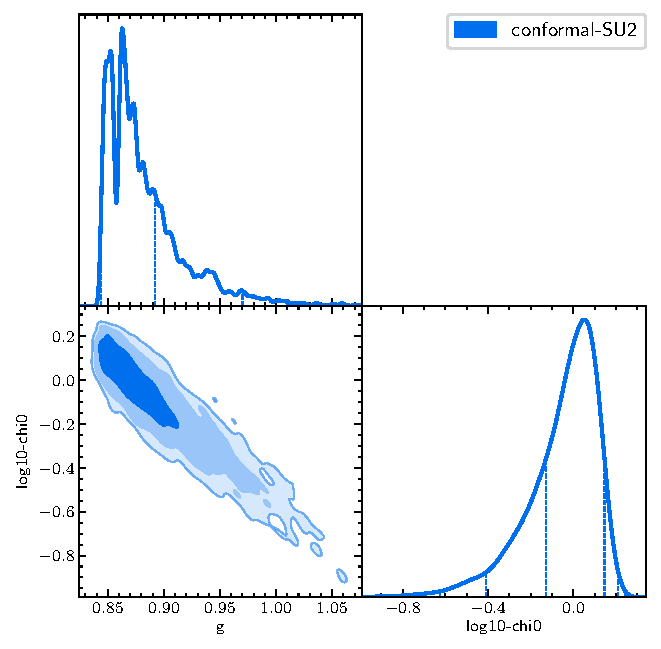
\includegraphics[width=0.9\textwidth]{conformal-SU2_posteriors.pdf}
\caption{Posterior distributions for $g$ and $\log_{10}(\chi_0/\text{GeV})$ from the PTArcade Bayesian analysis. Left: one-dimensional marginalised posteriors for each parameter. Right: two-dimensional joint posterior with $1\sigma$, $2\sigma$, and $3\sigma$ contours. The MAP point ($g=0.86$, $\log_{10}(\chi_0/\text{GeV})=0.049$) is marked.}
\label{fig:posteriors}
\end{figure}

Figure~\ref{fig:ptarcade_spectrum} shows the GW spectrum at the MAP point compared with the NANOGrav violin windows.

\begin{figure}[h]
\centering

\includegraphics[width=0.9\textwidth]{pta_ptarcade_spectrum.pdf}
\caption{Gravitational-wave spectrum at the PTArcade MAP point ($g=0.86$, $\chi_0=1.12$~GeV) overlaid on the NANOGrav 15-year violin windows. The MAP point sits inside the $1\sigma$ band for most frequency bins.}
\label{fig:ptarcade_spectrum}
\end{figure}

\subsection{Note on MAP vs.\ best scan points}

The MAP point ($\chi_0 = 1.12$~GeV) has a higher VEV than the best 14/14 benchmark points ($\chi_0 \approx 0.39$--$0.50$~GeV), which produces a GW peak at slightly lower frequency. This shift may reflect the prior volume effect: the MCMC explores a larger $\chi_0$ region than the benchmark grid, and the data are consistent with a range of $\chi_0$ values.

\section{Constraints}
\label{sec:constraints}

Eleven constraints were considered, as summarised in Table~\ref{tab:constraints}. Three are directly applicable, five require recasting from existing literature, two require dedicated new back-end modules, and one is not applicable.

\begin{table}[h]
\centering
\resizebox{\textwidth}{!}{
\begin{tabular}{clllc}
\toprule
ID & Constraint & Category & Applicability & Resolved? \\
\midrule
C01 & $\Delta N_{\text{eff}}$ from stable dark sector & $N_{\text{eff}}$ & Requires new backend & No \\
C02 & BBN bound on $T_{\text{reh}} > 1$~MeV & BBN & Direct & Partially \\
C03 & Dark matter overproduction & DM & Recast needed & No \\
C04 & Self-interacting DM (structure formation) & SIDM & Requires new backend & No \\
C05 & Fifth force on pseudo-dilaton & Other & Not applicable & Yes \\
C06 & Perturbativity ($g < 4\pi$) & Theory & Direct & Yes \\
C07 & CMB constraints on DM annihilation & CMB & Recast needed & No \\
C08 & Supernova cooling & SN & Recast needed & No \\
C09 & Higgs portal constraints & Collider & Recast needed & Yes \\
C10 & Eternal inflation & Theory & Direct & Yes \\
C11 & Dark photon / fixed-target searches & Beam dump & Recast needed & No \\
\bottomrule
\end{tabular}
}
\caption{Summary of considered constraints. ``Resolved'' means the constraint was either checked and found to be satisfied or determined to be inapplicable for the minimal model.}
\label{tab:constraints}
\end{table}

\subsection{Key constraints}

\paragraph{$\Delta N_{\text{eff}}$ (C01).} A stable dark SU(2) sector with 13 bosonic degrees of freedom (4 scalar + 9 vector) that was in thermal equilibrium with the SM contributes $\Delta N_{\text{eff}} \approx 0.64$ at BBN and CMB epochs, assuming all degrees of freedom are relativistic. The combined Planck+BBN bound is $\Delta N_{\text{eff}} < 0.18$ at 95\% CL~\cite{Yeh:2022}. If the dark sector was never in equilibrium with the SM, the constraint relaxes proportionally to $\xi^4 = (T_{\text{dark}}/T_{\text{SM}})^4$, but the exact dilution factor requires modelling the full thermal history including the FOPT reheating dynamics. Ref.~\cite{Bringmann:2023} found that stable dark sectors are strongly disfavoured as PTA explanations; decaying sectors (lifetime $\tau < 0.1$~s) remain viable.

\paragraph{BBN percolation (C02).} The best 14/14 benchmark points have $T_{\text{reh}} \approx 40$--$50$~MeV and the MAP point has $T_{\text{reh}} \approx 14.5$~MeV, safely satisfying the BBN bound $T_{\text{reh}} > 1$~MeV (or $T_{\text{reh}} > 3$~MeV for strong transitions~\cite{Bai:2022}). Marginal scan points with $T_p < \text{few}\times 0.1$~MeV would violate BBN.

\paragraph{Dark matter overproduction (C03).} The SU(2) gauge bosons are stable (mass $m_W \sim 0.3$--$0.6$~GeV in the $1\sigma$ region) and, without a decay or annihilation portal, would overclose the Universe via standard thermal freeze-out. Ref.~\cite{Frandsen:2023} finds that minimal SU(2) vector dark matter requires $m_V > 7.5$~TeV to avoid overproduction. The minimal model provides no mechanism to deplete the relic abundance; Ref.~\cite{Borah:2021} invoked a tiny Higgs portal ($\lambda_2 \sim 10^{-9}$) for freeze-in production, which avoids overproduction but does not address $\Delta N_{\text{eff}}$.

\section{Assumptions and Limitations}
\label{sec:assumptions}

The prior audit examined 42 assumptions, uncertainties, and limitations across five categories. Table~\ref{tab:audit_summary} summarises the severity distribution; Table~\ref{tab:critical_assumptions} lists the most critical unresolved items.

\begin{table}[h]
\centering
\begin{tabular}{lrr}
\toprule
Severity range & Total items & Controlled \\
\midrule
1--3 (Minor) & 14 & 11 \\
4--6 (Moderate) & 18 & 4 \\
7--8 (Significant) & 7 & 0 \\
9--10 (Critical) & 3 & 0 \\
\bottomrule
\end{tabular}
\caption{Severity distribution of the 42 audited assumptions. ``Controlled'' means the assumption was validated or its impact quantified.}
\label{tab:audit_summary}
\end{table}

\begin{table}[h]
\centering
\resizebox{\textwidth}{!}{
\begin{tabular}{clcl}
\toprule
ID & Severity & Description & Controlled? \\
\midrule
A08 & 6 & High-T expansion validity for strong supercooling & No \\
A14 & 6 & 29\% numerical failure rate in FOPT scan & No \\
A22 & 7 & Single MCMC chain, only 7501 effective samples & No \\
A25 & 6 & Eternal inflation criterion not validated vs.\ literature & No \\
A27 & 7 & $\alpha$ discrepancy with Borah et al.\ (factor 33) & No \\
A28 & 8 & $\Delta N_{\text{eff}}$ unresolved & No \\
A29 & 8 & DM overproduction unresolved & No \\
A37 & 7 & dbf template (arXiv:2511.15687) not verifiable & No \\
\bottomrule
\end{tabular}
}
\caption{Most critical unresolved assumptions and limitations.}
\label{tab:critical_assumptions}
\end{table}

Ten required follow-ups were identified. The highest-priority items are: (F01) a dedicated $\Delta N_{\text{eff}}$ calculation using the full FOPT thermal history; (F02) a relic abundance calculation for the SU(2) gauge bosons; (F03) cross-validation of the eternal inflation criterion against the standard literature condition; (F04) multiple MCMC chains with Gelman--Rubin convergence diagnostic; (F05) resolution of the $\alpha$ convention discrepancy; and (F06) verification or replacement of the dbf GW template.

\section{Discussion}
\label{sec:discussion}

\subsection{Caveats}

Several caveats must be acknowledged when interpreting these results.

First, the dbf GW template (referenced as arXiv:2511.15687) could not be verified through public searches at the time of this analysis. This paper may not yet be published or indexed. The template's validity for moderate $\alpha \sim \mathcal{O}(1\text{--}10)$ is acknowledged as less established. For strongly supercooled transitions ($\alpha \gg 1$), recent work~\cite{Caprini:2024a, Caprini:2024b} suggests that bubble collisions may dominate over sound waves, and the dbf template's treatment of this regime should be cross-validated.

Second, the GW spectra assume a secluded dark sector with no coupling to the Standard Model. This simplifies the analysis but makes the $\Delta N_{\text{eff}}$ constraint severe. Adding even a tiny portal (Higgs mixing or kinetic mixing) for dark sector decay before BBN would relax this constraint and may be phenomenologically required.

Third, the MCMC analysis uses a single chain with 7501 effective samples. Standard PTA analyses typically use 2--4 chains with Gelman--Rubin convergence diagnostics. While the posteriors appear plausible, a multi-chain analysis would improve confidence.

Finally, the model is identical to that studied by Borah et al.\ in 2021~\cite{Borah:2021}. Our independent analysis with newer data (NG15 vs.\ NG12.5) and updated computational tools (semianalytic pipeline, dbf template, PTArcade) broadly confirms that the conformal SU(2) dark sector can explain the PTA signal, though our preferred coupling ($g_{\text{MAP}} = 0.86$) is slightly smaller than their benchmark ($g_D = 1.37$).

\subsection{Comparison with literature}

\paragraph{arXiv:2109.11558 (Borah et al.)}~\cite{Borah:2021} studied exactly the same model for NANOGrav 12.5-yr data. Our $\beta/H$ agreement ($<1\%$) is excellent. The $\alpha$ discrepancy (ours 15 vs.\ theirs 0.45 at BP1) likely arises from different conventions for the radiation energy density denominator: our backend uses the full SM plus dark sector degrees of freedom, while Borah et al.\ may use a different normalisation. Our PTArcade posteriors ($g=0.86$, $\chi_0=1.12$~GeV) favour a larger VEV and smaller coupling than the Borah et al.\ BP1 ($g=1.37$, $\chi_0=0.012$~GeV), reflecting the different data set (NG15 vs.\ NG12.5) and GW template.

\paragraph{arXiv:2602.09092 (Bringmann et al.)}~\cite{Bringmann:2026} studied a structurally similar conformal U(1)$'$ model. Their best-fit point ($g=0.692$, $v=140$~MeV, $\alpha=821$, $\beta/H=57.9$) illustrates the typical parameter range for CW-type transitions. The SU(2) model produces stronger transitions (larger $\alpha$) due to the additional gauge degrees of freedom. The U(1)$'$ model is identified as the most generic, least tuned explanation; our SU(2) analysis extends this finding to the non-abelian case.

\paragraph{arXiv:2501.11619 (Goncalves et al.)}~\cite{Goncalves:2025} addresses percolation in supercooled conformal U(1)$'$ transitions, showing that the Euclidean action asymptotically approaches zero as $T\rightarrow 0$, guaranteeing percolation.

\section{Conclusions}
\label{sec:conclusions}

We have analysed the minimal classically scale-invariant SU(2)$_X$ gauge theory with one complex scalar doublet as an explanation of the nanohertz GW signal observed by NANOGrav. The model undergoes a strongly supercooled first-order phase transition via the Coleman--Weinberg mechanism, producing a GW spectrum consistent with the NANOGrav 15-year data.

Our main findings are:
\begin{itemize}
\item \textbf{Model viability}: The conformal SU(2)$_X$ model can fit the NANOGrav signal. Seven benchmark points achieve 14/14 in-violin bins at $g \approx 0.90$--$1.05$ and $\chi_0 \approx 0.39$--$0.50$~GeV.
\item \textbf{Bayesian posterior}: The MAP point is $g=0.86$, $\chi_0=1.12$~GeV, with $g$ constrained to $\lesssim 10\%$ relative width.
\item \textbf{Unresolved constraints}: The most serious unresolved issues are $\Delta N_{\text{eff}}$ from the stable dark sector (which likely requires a decay portal to the SM) and dark matter overproduction from stable gauge bosons.
\item \textbf{Assumptions}: An audit of 42 items identifies 10 required follow-ups, including dedicated $\Delta N_{\text{eff}}$ and relic abundance calculations, multi-chain MCMC, and GW template validation.
\end{itemize}

Answering the original question ``what is the minimal conformal non-abelian model that can explain the NANOGrav signal?'': the minimal classically scale-invariant SU(2) gauge theory with one complex scalar doublet is indeed a viable explanation, subject to unresolved cosmological constraints that require a decay portal to the Standard Model. The model is not novel (it was studied by Borah et al.\ in 2021), but our updated analysis confirms its compatibility with the NG15 data and provides new Bayesian posterior constraints.

\begin{thebibliography}{50}

\bibitem{Pascoli:2026}
S.~Pascoli, S.~Rosauro-Alcaraz, M.~Zandi,
``Cosmological phase transitions: from particle physics to gravitational waves, semi-analytically,''
arXiv:2602.02829 [hep-ph].

\bibitem{Bringmann:2026}
T.~Bringmann, T.~Konstandin, J.~Matuszak, K.~Schmidt-Hoberg, C.~Tasillo,
``Tuning the violins: dark sector phase transition models for the PTA signal,''
arXiv:2602.09092 [hep-ph].

\bibitem{Borah:2021}
D.~Borah, A.~Dasgupta, S.~K.~Kang,
``A first order dark SU(2)$_D$ phase transition with vector dark matter in the light of NANOGrav 12.5 yr data,''
JCAP \textbf{12} (2021) 037, arXiv:2109.11558 [hep-ph].

\bibitem{Bringmann:2023}
T.~Bringmann, P.~F.~Depta, T.~Konstandin, K.~Schmidt-Hoberg, C.~Tasillo,
``Does NANOGrav observe a dark sector phase transition?,''
JCAP \textbf{11} (2023) 053, arXiv:2306.09411 [hep-ph].

\bibitem{Agazie:2023}
G.~Agazie \textit{et al.} (NANOGrav Collaboration),
``The NANOGrav 15-year Data Set: Evidence for a Gravitational-Wave Background,''
Astrophys. J. Lett. \textbf{951} (2023) L8, arXiv:2306.16213 [astro-ph.HE].

\bibitem{Coleman:1973}
S.~R.~Coleman and E.~J.~Weinberg,
``Radiative Corrections as the Origin of Spontaneous Symmetry Breaking,''
Phys. Rev. D \textbf{7} (1973) 1888--1910.

\bibitem{DBFtemplate}
Dissipative bulk-flow GW template,
arXiv:2511.15687 [hep-ph].
\textit{(Note: this reference could not be verified through public searches at the time of writing.)}

\bibitem{Mitridate:2023}
A.~Mitridate \textit{et al.},
``PTArcade: A fast Bayesian analysis pipeline for PTA data,''
arXiv:2306.16377 [astro-ph.HE].

\bibitem{Yeh:2022}
T.-H.~Yeh, K.~A.~Olive, B.~D.~Fields,
``Probing Physics Beyond the Standard Model: Limits from BBN and the CMB Independently and Combined,''
JCAP \textbf{03} (2023) 046, arXiv:2207.13133 [astro-ph.CO].

\bibitem{Bai:2022}
Y.~Bai and M.~Korwar,
``BBN constraints on MeV-scale phase transitions,''
JHEP \textbf{02} (2022) 184, arXiv:2109.14765 [hep-ph].

\bibitem{Frandsen:2023}
M.~T.~Frandsen, J.~S.~Heinesen, M.~Rosenlyst, S.~K.~B.~Svensson,
``Minimal SU(2) vector dark matter,''
Phys. Rev. D \textbf{107} (2023) 115023, arXiv:2301.00041 [hep-ph].

\bibitem{Goncalves:2025}
J.~Goncalves, D.~Marfatia, A.~P.~Morais, R.~Pasechnik,
``Supercooled phase transitions in conformal dark sectors explain NANOGrav data,''
Phys. Lett. B \textbf{869} (2025) 139829, arXiv:2501.11619 [hep-ph].

\bibitem{Caprini:2024a}
C.~Caprini, R.~Jinno, T.~Konstandin, A.~Roper Pol, H.~Rubira, I.~Stomberg,
``Gravitational waves from first-order phase transitions: from weak to strong,''
arXiv:2409.03651 [astro-ph.CO].

\bibitem{Caprini:2024b}
C.~Caprini \textit{et al.},
``Science with the space-based interferometer eLISA. II: Gravitational waves from cosmological phase transitions,''
JCAP \textbf{04} (2016) 001, arXiv:1512.06239 [astro-ph.CO].

\bibitem{Sagunski:2021}
L.~Sagunski, S.~Gad-Nasr, B.~Colquhoun, A.~Robertson, S.~Tulin,
``Velocity-dependent Self-interacting Dark Matter from Groups and Clusters of Galaxies,''
JCAP \textbf{01} (2021) 024, arXiv:2006.12515 [astro-ph.CO].

\bibitem{Damour:2010}
T.~Damour and J.~F.~Donoghue,
``Equivalence Principle Violations and Couplings of a Light Dilaton,''
Phys. Rev. D \textbf{82} (2010) 084033, arXiv:1007.2792 [gr-qc].

\bibitem{Slatyer:2016}
T.~R.~Slatyer,
``Indirect dark matter signatures in the cosmic dark ages. I. Generalizing the bound on s-wave dark matter annihilation from Planck results,''
Phys. Rev. D \textbf{93} (2016) 023527, arXiv:1512.06239 [hep-ph].

\bibitem{BaBar:2017}
J.~P.~Lees \textit{et al.} (BaBar Collaboration),
``Search for Invisible Decays of a Dark Photon Produced in $e^+e^-$ Collisions at BaBar,''
Phys. Rev. Lett. \textbf{119} (2017) 131804, arXiv:1702.03327 [hep-ex].

\bibitem{Kierkla:2023}
M.~Kierkla, A.~Karam, B.~Swiezewska,
``Conformal model for gravitational waves and dark matter: A status update,''
JHEP \textbf{03} (2023) 007, arXiv:2210.07075 [hep-ph].

\end{thebibliography}

\end{document}